\documentclass{article}

\usepackage[utf8]{inputenc}
\usepackage{graphicx}
\usepackage{listings}
\usepackage{color}
\usepackage{float}

\definecolor{dkgreen}{rgb}{0,0.6,0}
\definecolor{gray}{rgb}{0.5,0.5,0.5}
\definecolor{mauve}{rgb}{0.58,0,0.82}

\lstset{frame=tb,
    language=C,
    aboveskip=3mm,
    belowskip=3mm,
    showstringspaces=false,
    columns=flexible,
    basicstyle={\small\ttfamily},
    numbers=left,
    numberstyle=\tiny\color{gray},
    keywordstyle=\color{blue},
    commentstyle=\color{dkgreen},
    stringstyle=\color{mauve},
    breaklines=true,
    breakatwhitespace=true,
    tabsize=3
}


\title{TP2 IA: Logique floue}
\date{\today}
\author{ABDELMOUMENE Djahid}

\begin{document}
\maketitle

\section{Implementation de moteur d'inférence}

pour le moteur d'inférence j'ai créé une petite API qui a toutes les fonctions
nécessaires pour créer des variables linguistiques, des fonctions
d'appartenance et des règles. tout cela peut être placé dans une autre
structure appelée \textit{FUZZY\_SYS} qui a les deux variables d'entrée et une
variable de sortie, une liste des fonctions d'appartenance pour stocker la
sortie de l'inférence et la liste des règles floue.
\begin{lstlisting}
typedef struct fuzzy_logic_system {
   IN_LING_VAR *x, *y; // les variables d'entrees
   OUT_LING_VAR *z;    // les variables de sortie

   // pour stocker la liste des fonctions d'appartenance
   // on prend le maximum de toutes ces fonctions pour chaque valeur de x
   FUZZY_SET_LIST* out;

   // les regles floues
   FUZZY_RULE* rules;
} FUZZY_SYS;
\end{lstlisting}


Chaque fonction d'appartenance ou ensemble flou est défini comme un trapèze,
nous avons donc besoin des quatre valeurs x des points du trapèze et une
hauteur, la structure appelé \textit{FUZZY\_SET} ressemble à ceci :
\begin{lstlisting}
struct fuzzy_set {
   char *set_name; // the set's linguistic name eg: 'hot', 'far' etc..

   float x1;
   float x2;
   float x3;
   float x4;

   float height;
};
\end{lstlisting}

Les variables linguistique sont definis avec un valeur min et max de x, ça sera
utile aprés lors de la defuzzification, le struct contient aussi toutes les
fonctions d'appartenance possible pour ce variable, avec une valeur d'entree
pour les variables d'entree:

\begin{lstlisting}
struct linguistic_variable {
   char *var_name; // variable name
   float min_x;                   // start of the x range
   float max_x;                   // end of the x range

   float input; // seulement pour les variables d'entree

   // FUZZY_SET_LIST est une liste chainee de fonctions d'appartenance
   FUZZY_SET_LIST* fuzzy_sets;  // list of fuzzy sets
};
\end{lstlisting}

Les régles floues sont définis par les trois fonctions d'appartenance des
variables d'entrees et de sortie. Et c'est sous forme d'une liste chainée pour
faciliter l'ajour des nouvelles regles

\begin{lstlisting}
typedef struct fuzzy_rule {
   FUZZY_SET *A, *B, *C; // fuzzy sets of rule definition

   FUZZY_RULE* next;  // next fuzzy rule
} FUZZY_RULE;
\end{lstlisting}


pour le processus d'inférence, il y a trois étapes, la fuzzification, puis
l'inférence réelle et la défuzzification, la première étape - la fuzzification
- consiste à définir la variable linguistique appropriée du système avec la
bonne valeur de saisie. \\

Ensuite, pour l'inférence, nous prenons les valeurs d'entrée pour chacune des
deux variables linguistiques d'entrée, nous parcourons toutes les règles
floues de systéme, puis on calcule les fonctions d'appartenance aux entrées (A
et B) 
fournies pour les deux premiers ensembles de la règle courante, et en prenant le
minimum, nous prenons ensuite le dernier ensemble (C) dans la règle et on fait
un clipping de la hauteur, qui devient maintenant le minimum précédent que nous avons calculé.
Pour faire le clipping, nous devons recalculer les valeurs x des deuxième
et troisième points du trapèze de la fonction d'appartenance (C). Pour tous ces
points, nous construisons une liste de ces trapézes résultants que nous stockons
ensuite dans le champ \textit{out} de la structure \textit{FUZZY\_SYS}. \\

La dernière étape est la défuzzification dans laquelle nous prenons le résultat
de l'étape précédente -liste des trapèzes- et nous trouvons le centre de masse
de la forme que nous obtenons lorsqu'on prend les maximums de tous ces
trapèzes. Pour ce faire, nous parcourants toutes les valeurs x de
\textit{min\_x}
(champ de la variable linguistique) à \textit{max\_x}, et calculons à chaque étape le
maximum de toutes les valeurs de tous les ensembles dans le x courant, puis nous utilisons ces
valeurs pour calculer la surface du trapèze obtenu, puis nous la multiplions
par la valeur x courante. nous prenons la somme de toutes ces surfaces
pondérées et des surfaces régulières. En fin de compte, le centre de mass résultant
est la somme pondérée divisée par la surface totale. \\

Cette valeur qu'on a obtenue est la valeurs 'crisp' de variable de sortie qu'on
cherche.

\begin{figure}
  \centering
      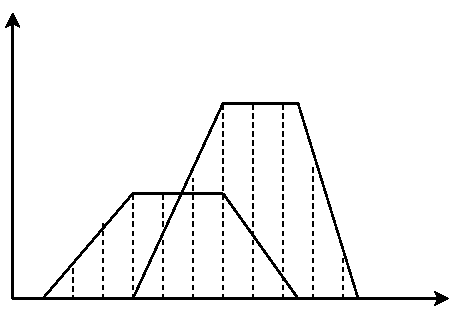
\includegraphics[width=0.5\textwidth]{defuzz.pdf}
  \caption{Les trapézes qu'on obtient à chaque itération sont dessiné avec des
   lignes de pointillés}
\end{figure}


\section{L'application}

Pour utiliser l'API sur le probleme donnée j'ai créer 4 variables linguistique,
2 pour les capteurs gauche et droite et deux pour les deux moteurs. Les
variables des capteurs peuvent avoir 3 differents états 'close', 'half' ou
'far', qui sont les distance en forme linguistique, voici les definitions de ces
fonctions d'appartenance:
\begin{figure} [H]
  \centering
      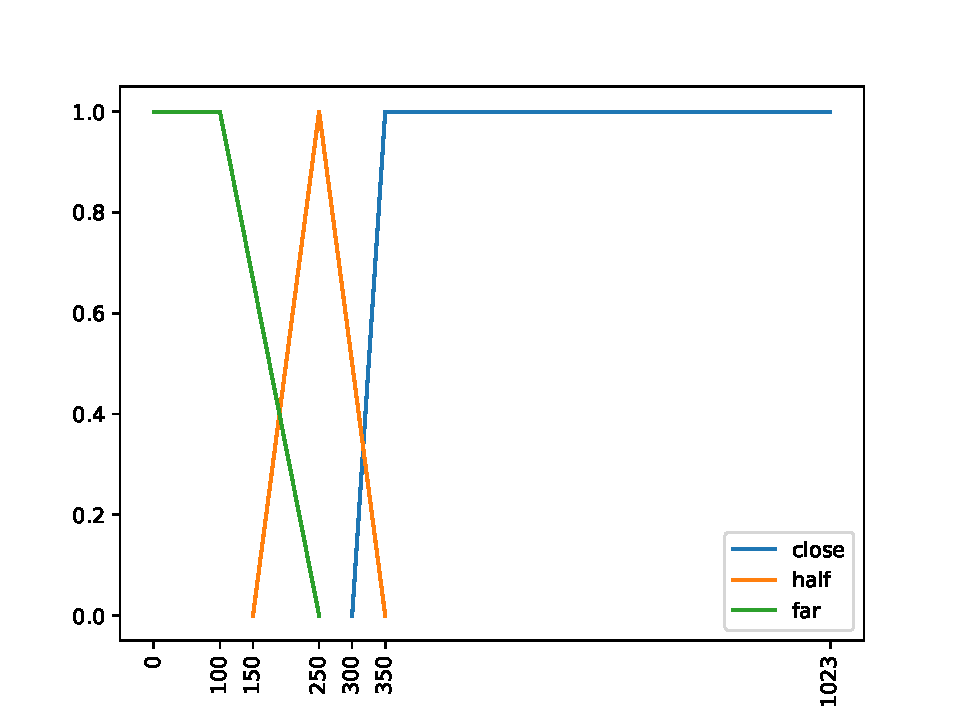
\includegraphics[width=0.5\textwidth]{sensor.pdf}
  \caption{Les fonctions d'appartenance pour les variables des capteurs}
\end{figure}

Pour les moteurs il existe aussi 3 differents états:
\begin{figure} [H]
  \centering
      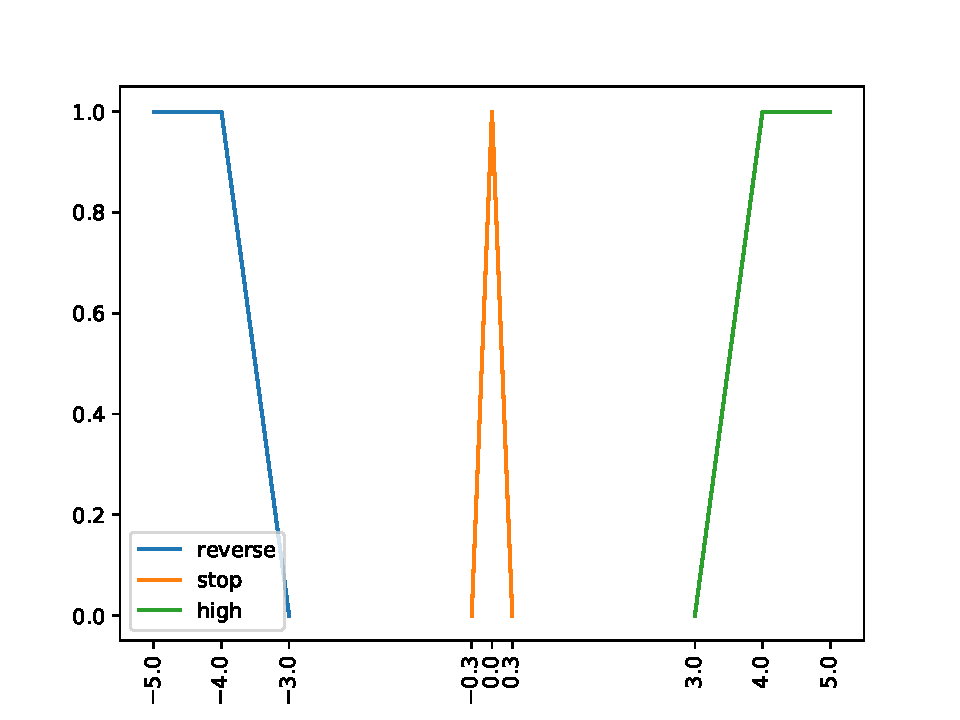
\includegraphics[width=0.5\textwidth]{motor.pdf}
  \caption{Les fonctions d'appartenance pour les variables des moteurs}
\end{figure}

Pour génerer les vitesses de chaque moteurs, j'ai utiliser deux systémes
d'inference, un pour chaque moteur. voici les régles pour le moteur gauche:
\begin{itemize}
   \item Si le mur à gauche est proche et à droite c'est loin alors arrêter.
   \item Si le mur à gauche est loin et à droite c'est proche alors accélerer.
   \item Si les deux murs sont loin alors accélerer.
   \item Si les deux murs sont proche mais un des deux c'est plus loin que
      l'autre alors accélerer en arriére si c'est l'un a gauche est plus proche
      sinon accélerer normalement.
\end{itemize}

Les régles de moteur droite sont l'inverse de ces régles.
\end{document}
